\documentclass[12pt, a4paper]{article}

\usepackage[utf8]{inputenc}
\usepackage[T1]{fontenc}
\usepackage[spanish]{babel}
\usepackage{geometry}
\usepackage{graphicx}
\usepackage{hyperref}
\usepackage{listings}
\usepackage{xcolor}
\usepackage{float}
\usepackage{caption}
\usepackage{subcaption}
\usepackage{amsmath}
\usepackage{booktabs}
\usepackage{array}
\usepackage{parskip}
\usepackage{fancyhdr}

\geometry{a4paper, top=3cm, bottom=2.5cm, left=3cm, right=2.5cm}
\graphicspath{{../media/}}

\hypersetup{
    colorlinks=true,
    linkcolor=black!60!black,
    urlcolor=blue!60!black,
    citecolor=green!50!black,
    pdftitle={Lane Keeping Control: Detección de Carriles y Seguimiento de Carril},
    pdfauthor={Agustín Mayor, Rafael Muñoz, José Francisco López},
}

\definecolor{codegreen}{rgb}{0,0.6,0}
\definecolor{codegray}{rgb}{0.5,0.5,0.5}
\definecolor{codepurple}{rgb}{0.58,0,0.82}
\definecolor{backcolour}{rgb}{0.97,0.97,0.97}
\lstdefinestyle{mystyle}{
    backgroundcolor=\color{backcolour},
    commentstyle=\color{codegreen}, keywordstyle=\color{blue},
    numberstyle=\tiny\color{codegray}, stringstyle=\color{codepurple},
    basicstyle=\ttfamily\footnotesize, breaklines=true,
    keepspaces=true, numbers=left, numbersep=5pt,
    showstringspaces=false, tabsize=2, frame=single,
    rulecolor=\color{gray!30}
}
\lstset{style=mystyle}

\pagestyle{fancy}
\fancyhf{}
\rhead{Control en Vehículos -- MIERA 2025/26}
\lhead{Detección y Seguimiento de Carril}
\cfoot{\thepage}

% ─────────────────────────────────────────────────────────────────────────────
\begin{document}
% ─────────────────────────────────────────────────────────────────────────────

\begin{titlepage}
    \centering
    \vspace*{2cm}
    {\large Universidad de Sevilla \par}
    {\large Máster en Ingeniería de Electrónica, Robótica y Automática (MIERA) \par}
    \vspace{1cm}
    {\large Control en Vehículos \par}
    \vspace{2cm}
    \hrule\vspace{0.5cm}
    {\Huge\bfseries Detección de Carriles y Control de Mantenimiento de Carril \par}
    \vspace{0.5cm}\hrule
    \vspace{2cm}
    {\large\itshape Grupo 1 \par}
    \vspace{1cm}
    \begin{tabular}{l}
        Agustín Mayor \\[4pt]
        Rafael Muñoz  \\[4pt]
        José Francisco López
    \end{tabular}
    \vfill
    {\large Curso 2025--2026 \par}
\end{titlepage}

\tableofcontents
\newpage

\begin{abstract}
    Este trabajo presenta el diseño e implementación de un sistema de \textit{Lane Keeping Assist} (LKA) para un vehículo autónomo simulado en \textit{CARLA Simulator} e integrado con \textit{ROS2 Humble} mediante contenedores Docker. El sistema consta de tres bloques principales: detección de líneas de carril mediante visión clásica con OpenCV y la transformada de Hough, diseño y sintonización de un controlador PID para mantener el vehículo centrado en el carril, y la integración de ambos módulos en un entorno de simulación realista donde se valida el funcionamiento completo. El código fuente, datasets e imágenes y vídeos demostrativos están disponibles en el repositorio público de GitHub: \url{https://github.com/JoseLopez36/Deteccion-Seguimiento-Carril}.
\end{abstract}

\newpage

% ═════════════════════════════════════════════════════════════════════════════
\section{Introducción}
% ═════════════════════════════════════════════════════════════════════════════

Los sistemas de asistencia a la conducción (ADAS) son hoy en día un componente fundamental tanto en la industria del automóvil como en la investigación en robótica móvil. Entre estos sistemas destaca el \textit{Lane Keeping Assist} (LKA), cuyo objetivo es mantener el vehículo centrado en su carril de forma autónoma, corrigiendo continuamente la dirección en función de la posición relativa del vehículo respecto a las marcas viales.

Este trabajo aborda el diseño e implementación de un sistema LKA completo, desde la adquisición de imagen hasta la actuación sobre los mandos del vehículo, validado en el simulador \textit{CARLA Simulator} mediante \textit{ROS2 Humble}. El flujo de funcionamiento del sistema es el siguiente:

\begin{enumerate}
    \item Adquisición de imágenes desde la cámara RGB frontal del vehículo simulado.
    \item Preprocesado de la imagen y detección de las líneas del carril mediante visión clásica.
    \item Cálculo del error lateral del vehículo respecto al centro del carril, expresado en metros a partir de los parámetros intrínsecos de la cámara.
    \item Generación de los comandos de aceleración/frenado y dirección mediante controladores PID, sintonizados previamente en MATLAB/Simulink.
    \item Publicación de los comandos de control al simulador CARLA.
\end{enumerate}

Todo el código fuente, datasets y material multimedia están disponibles en el repositorio público de GitHub del proyecto:
\begin{center}
    \url{https://github.com/JoseLopez36/Deteccion-Seguimiento-Carril}
\end{center}

\subsection*{Estructura de la memoria}

La memoria se organiza en tres bloques principales:

\begin{description}
    \item[Sección \ref{sec:carriles}: Detección de carriles.]
          Describe el pipeline de visión artificial empleado para detectar las marcas viales y calcular el error lateral del vehículo.
    \item[Sección \ref{sec:control}: Control de mantenimiento de carril.]
          Explica el modelado del vehículo y la sintonización del controlador PID en MATLAB/Simulink.
    \item[Sección \ref{sec:integracion}: Integración en simulación y resultados.]
          Desarrolla la arquitectura software completa en CARLA/ROS2, la infraestructura Docker, los nodos implementados y los resultados obtenidos.
\end{description}

% ═════════════════════════════════════════════════════════════════════════════
\section{Detección de carriles}
\label{sec:carriles}
% ═════════════════════════════════════════════════════════════════════════════

La detección de carriles constituye la capa de percepción del sistema LKA, encargada de transformar cada \textit{frame} de la cámara frontal en una estimación numérica de la posición lateral del vehículo dentro de su carril. El módulo se ha implementado mediante técnicas de visión clásica con OpenCV, evitando el uso de redes neuronales para mantener un pipeline ligero, interpretable y ejecutable en tiempo real sin necesidad de GPU dedicada ni de un dataset de entrenamiento.

\subsection{Pipeline de procesamiento de imagen}

El detector recibe la imagen RGB de la cámara frontal y aplica una secuencia de etapas clásicas de visión artificial para aislar las marcas viales y ajustar una línea representativa a cada lado del carril:

\begin{enumerate}
	\item \textbf{Realce de color.} La imagen se convierte al espacio de color HLS(\textit{Hue-Lightness-Saturation}), en el que se aplican dos umbralizaciones independientes: una para marcas blancas (alta luminosidad) y otra para marcas amarillas (rango de tono específico). La unión de ambas máscaras aísla los píxeles candidatos a pertenecer a una línea de carril, independientemente de su color. Trabajar en HLS hace que la detección sea mucho más estable.
	\item \textbf{Conversión a escala de grises y suavizado.} La imagen se convierte a escala de grises y se enmascara con el resultado del paso anterior, de forma que únicamente los píxeles de marca vial conservan información. A continuación se aplica un filtro \textit{Gaussian Blur} para atenuar el ruido de alta frecuencia (como imperfecciones en el asfalto) antes de la detección de bordes.
	\item \textbf{Detección de bordes (Canny).} Se aplica el detector de bordes de Canny sobre la imagen suavizada, con umbrales bajo y alto configurables (\texttt{canny\_low}, \texttt{canny\_high}), obteniendo un mapa binario de contornos.
	\item \textbf{Región de interés (ROI).} Se enmascara la imagen de bordes con un polígono trapezoidal que delimita la zona de carretera frente al vehículo, descartando el cielo, los laterales y otros elementos de la escena ajenos al carril. La altura del horizonte del trapecio es configurable mediante el parámetro \texttt{horizon}.
	\item \textbf{Transformada de Hough probabilística.} Sobre los bordes filtrados por el ROI se ejecuta \texttt{cv2.HoughLinesP}, que detecta segmentos de recta caracterizados por su resolución angular y de distancia, el número mínimo de votos (\texttt{hough\_threshold}), la longitud mínima de segmento (\texttt{hough\_min\_len}) y el hueco máximo tolerado dentro de un mismo segmento (\texttt{hough\_max\_gap}).
	\item \textbf{Clasificación y ajuste por lado.} Cada segmento detectado se clasifica como perteneciente a la línea izquierda o derecha del carril según el signo de su pendiente, descartando previamente los segmentos casi horizontales mediante el umbral \texttt{min\_slope}. Los puntos de cada lado se ajustan mediante una regresión lineal (\texttt{numpy.polyfit}) que produce una única recta representativa por lado, extrapolada entre la base de la imagen y la altura del horizonte definida por el ROI.
	\item \textbf{Suavizado temporal.} Las coordenadas de cada línea se promedian con las de los últimos \texttt{smoothing} \textit{frames} mediante una cola de tipo FIFO, lo que reduce el parpadeo de la detección frame a frame y aporta estabilidad ante oclusiones puntuales o segmentos de Hough erróneos.
\end{enumerate}

Todos los parámetros del pipeline se agrupan en una estructura de configuración (\texttt{LaneConfig}), lo que permite ajustar el comportamiento del detector --umbrales de Canny, parámetros de Hough, pendiente mínima, ventana de suavizado y altura del horizonte-- sin modificar el código, cargándolos como parámetros ROS2 en tiempo de ejecución.

\subsection{Cálculo de la posición lateral}

A partir de las líneas izquierda y derecha ajustadas, el detector estima la posición lateral del vehículo dentro del carril evaluando ambas rectas en la fila inferior de la imagen (la más cercana al vehículo). Se distinguen tres casos:

\begin{itemize}
	\item \textbf{Ambas líneas detectadas.} Se calcula el centro del carril como el punto medio entre las coordenadas $x$ de ambas líneas en la base de la imagen, y la anchura del carril como su diferencia. El desplazamiento lateral en píxeles (\texttt{offset\_px}) se obtiene como la diferencia entre el centro geométrico de la imagen y el centro del carril. Adicionalmente se define una magnitud normalizada \texttt{lateral} $\in [0, 1]$, que representa la posición relativa del centro de la imagen respecto a las dos líneas (0 sobre la línea izquierda, 0.5 en el centro exacto del carril, 1 sobre la línea derecha).
	\item \textbf{Solo una línea detectada.} Si únicamente se detecta uno de los dos lados --situación habitual en curvas pronunciadas o marcas viales discontinuas--, el desplazamiento lateral se aproxima respecto a la línea visible, asumiendo que el vehículo se aleja de ella en la dirección del lado no detectado.
	\item \textbf{Ninguna línea detectada.} El estado se marca como \texttt{UNKNOWN} y no se actualiza el error lateral, manteniéndose el último valor válido hasta la recuperación de la detección.
\end{itemize}

A partir del valor normalizado \texttt{lateral} se clasifica la posición del vehículo en una de tres zonas discretas, en función de un umbral de centrado configurable (\texttt{center\_threshold}, fijado en 0.20): \texttt{LEFT} si el vehículo está desplazado hacia la línea izquierda más allá del umbral, \texttt{RIGHT} si lo está hacia la derecha, y \texttt{CENTER} en caso contrario. Esta clasificación por zonas, sumada al valor continuo de \texttt{offset\_px}, permite tanto generar alertas discretas de cruce o cambio de carril como alimentar un controlador continuo de mantenimiento de carril.

\subsection{Conversión a unidades métricas}

El error lateral calculado por el pipeline de visión se expresa inicialmente en píxeles, una unidad dependiente de la resolución y la óptica de la cámara. Para emplear dicho error como señal de referencia de un controlador físico es necesario expresarlo en metros, unidad utilizada en el modelo cinemático del vehículo (Sección~\ref{sec:control}).

La conversión se realiza a partir de la longitud focal $f_x$ de la cámara, obtenida del mensaje \texttt{camera\_info} publicado por el simulador (elemento $K_{00}$ de la matriz intrínseca). El error lateral en metros se aproxima como:

\begin{equation}
	e_{\text{lateral}}~\text{[m]} = \frac{\texttt{offset\_px}}{f_x}
\end{equation}

Esta aproximación asume una proyección de perspectiva simple y es válida bajo la hipótesis de que el plano de la carretera es aproximadamente perpendicular al eje óptico en la región de interés cercana al vehículo. Hasta que el nodo de detección recibe el primer mensaje de \texttt{camera\_info}, el error se publica directamente en píxeles como valor de respaldo.

\subsection{Salida del módulo de detección}

El detector expone su resultado mediante una estructura de estado (\texttt{LaneState}) que recoge, para cada \textit{frame} procesado: la zona de posición (\texttt{CENTER}/\texttt{LEFT}/\texttt{RIGHT}/\texttt{UNKNOWN}), el valor normalizado \texttt{lateral}, el desplazamiento \texttt{offset\_px}, la anchura estimada del carril en píxeles y los indicadores booleanos de detección de cada línea. Esta estructura constituye la interfaz entre el módulo de percepción y el resto del sistema, y es la que consume el nodo \texttt{lane\_detection\_node} (Sección~\ref{sec:integracion}) para publicar el error lateral y el estado del carril como mensajes ROS2.

% ─────────────────────────────────────────────────────────────────────────────
\subsection{Pruebas previas sobre vídeo real}
% ─────────────────────────────────────────────────────────────────────────────

Antes de integrar el detector en el simulador CARLA, el pipeline descrito en las secciones anteriores se validó de forma independiente sobre vídeo real de carretera, ejecutando el módulo de detección como aplicación \textit{standalone} en Python sobre secuencias grabadas desde un vehículo. Esta etapa de prueba permitió ajustar los parámetros del pipeline --umbrales de Canny, ventana de suavizado y altura del horizonte del ROI-- en un escenario con condiciones de iluminación e infraestructura viaria distintas a las del entorno sintético de CARLA, antes de invertir tiempo en la integración con ROS2 y el simulador.

La Figura~\ref{fig:prueba_video} muestra un fotograma representativo de estas pruebas, en el que se observa el polígono de carril superpuesto en verde semitransparente, las líneas izquierda (azul) y derecha (amarilla) ajustadas mediante regresión lineal, y el panel de telemetría con la zona de posición, el valor normalizado \texttt{lateral} y el desplazamiento en píxeles. 

\begin{figure}[H]
	\centering
	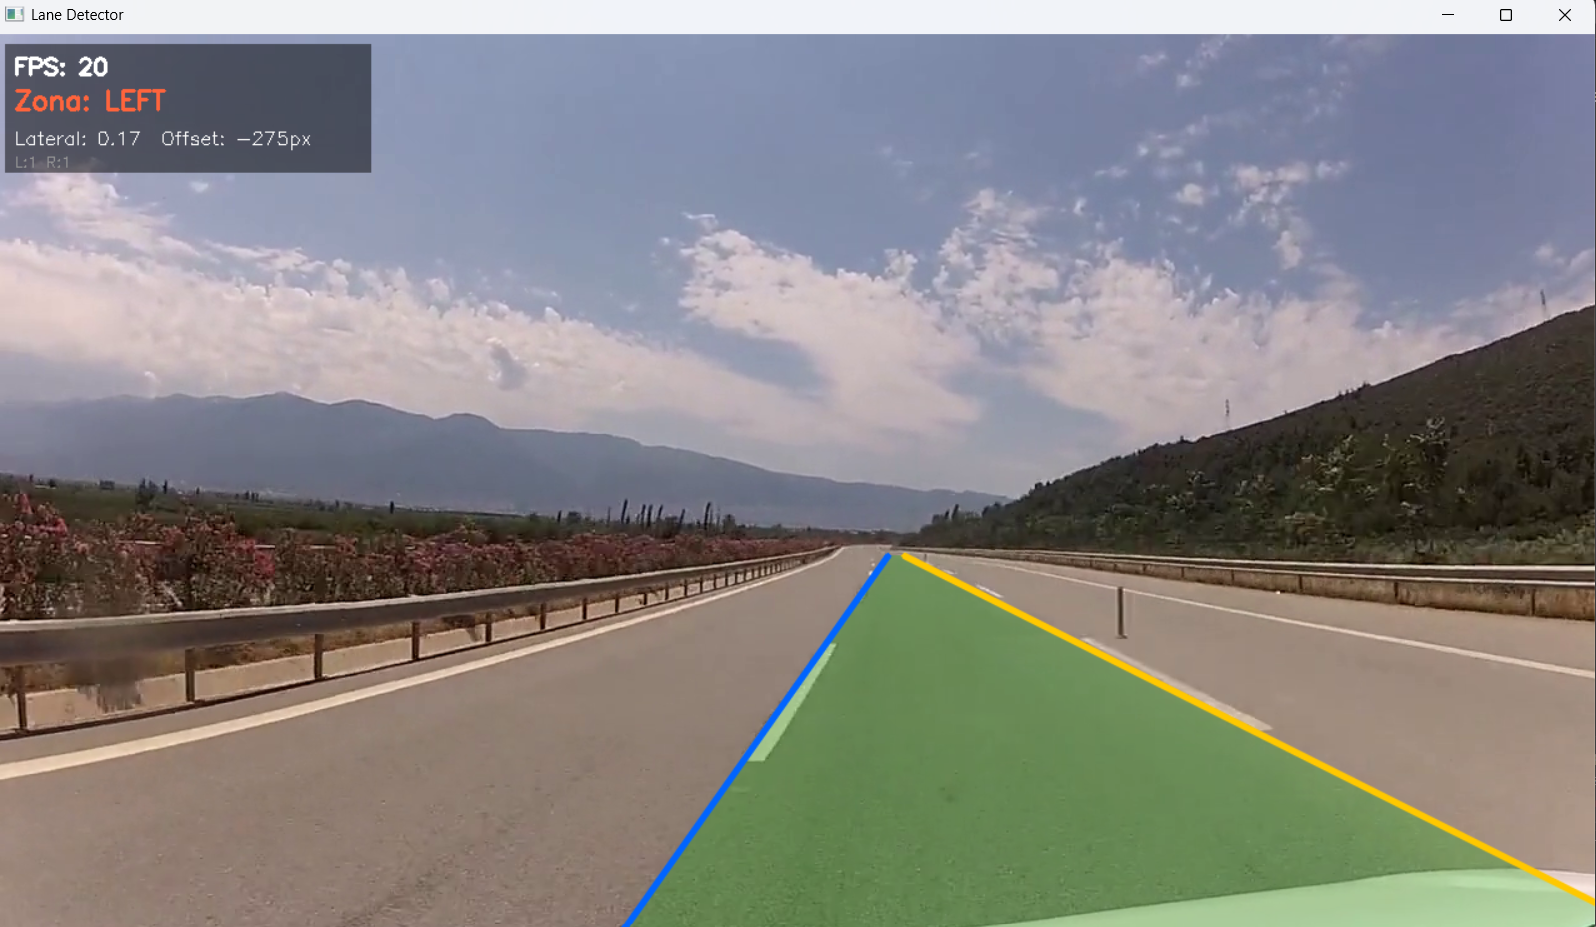
\includegraphics[width=0.70\textwidth]{Prueba_Video_Previa.png}
	\caption{Fotograma de las pruebas previas del detector de carriles sobre vídeo real de carretera, mostrando el polígono de carril, las líneas ajustadas y el panel de telemetría con la zona de posición (\texttt{LEFT}) y el desplazamiento lateral.}
	\label{fig:prueba_video}
\end{figure}

Los resultados obtenidos sobre vídeo real confirmaron la viabilidad del pipeline de visión clásica antes de su traslado al entorno simulado, validando en particular la robustez del ajuste por regresión lineal y del suavizado temporal frente al ruido visual propio de una escena no controlada (variaciones de iluminación, vegetación lateral y marcas viales parcialmente desgastadas).

% ═════════════════════════════════════════════════════════════════════════════
\section{Control de mantenimiento de carril}
\label{sec:control}
% ═════════════════════════════════════════════════════════════════════════════

Esta sección describe el modelado del vehículo y el proceso de diseño y sintonización del controlador PID de dirección empleado para el mantenimiento de carril. El flujo de diseño sigue la metodología clásica de control: primero se establece un modelo dinámico del sistema, después se sintoniza el controlador en MATLAB/Simulink y, finalmente, los parámetros obtenidos se transfieren directamente a la implementación en Python/ROS2 descrita en la Sección~\ref{sec:integracion}.

% ─────────────────────────────────────────────────────────────────────────────
\subsection{Modelado del vehículo}
% ─────────────────────────────────────────────────────────────────────────────


Para el diseño del controlador de dirección se adopta un modelo cinemático de vehículo tipo bicicleta (\textit{bicycle model}), ampliamente utilizado en aplicaciones de control lateral por su equilibrio entre fidelidad y manejabilidad analítica. En este modelo el vehículo queda descrito por su posición lateral $y$, su ángulo de guiñada $\psi$ y el ángulo de dirección de las ruedas delanteras $\delta$.

El error de seguimiento de carril se define como el desplazamiento lateral del punto central del eje delantero respecto al centro del carril, calculado a partir de la imagen de la cámara frontal tal como se describe en la Sección~\ref{sec:carriles}. Este error, expresado en metros, es la señal de referencia del bucle de control de dirección.

El modelo del vehículo simulado en MATLAB/Simulink toma como referencia los parámetros dinámicos del vehículo disponible en el entorno de simulación, siguiendo el mismo esquema que el ego-vehicle empleado en CARLA (Tesla Model 3). Los parámetros relevantes del modelo son la distancia entre ejes (\textit{wheelbase}) $L$ y la velocidad de avance $v$, que se trata como perturbación paramétrica durante la sintonización dado que el controlador de crucero la regula de forma independiente (véase la Sección~\ref{sec:integracion}).

% ─────────────────────────────────────────────────────────────────────────────
\subsection{Estructura de control en cascada}
% ─────────────────────────────────────────────────────────────────────────────

El sistema de control se organiza en dos lazos independientes que operan en cascada:

\begin{enumerate}
    \item \textbf{Lazo externo — control de velocidad (PI):} regula la velocidad longitudinal del vehículo en torno a la referencia deseada $v_\text{ref}$, actuando sobre el acelerador y el freno.
    \item \textbf{Lazo interno — control de dirección (PID):} emplea el error lateral $e_s$ proporcionado por el módulo de detección de carriles para calcular el ángulo de volante corrector y mantener el vehículo centrado en el carril.
\end{enumerate}

Esta arquitectura en cascada permite diseñar y sintonizar cada lazo de forma independiente, aprovechando la separación de escalas temporales entre la dinámica longitudinal (lenta) y la lateral (más rápida).

% ─────────────────────────────────────────────────────────────────────────────
\subsection{Sintonización en MATLAB/Simulink}
% ─────────────────────────────────────────────────────────────────────────────

El proceso de sintonización se realiza íntegramente en MATLAB/Simulink antes de trasladar los parámetros al entorno ROS2/CARLA. El diagrama de bloques del modelo incluye: el generador de error lateral de referencia, el bloque PID de dirección, el modelo cinemático del vehículo y el bloque de realimentación que cierra el lazo.

Para evaluar la respuesta del controlador se inyecta un error lateral artificial en el punto de entrada del PID. Esta estrategia permite explorar la respuesta transitoria del sistema ante perturbaciones de posición sin necesidad de una trayectoria de referencia compleja, facilitando el ajuste iterativo de las ganancias.

Las ganancias se sintonizaron siguiendo un proceso manual asistido por la herramienta \texttt{pidTuner} de MATLAB, imponiendo los siguientes criterios de diseño:

\begin{itemize}
    \item Tiempo de establecimiento reducido: el vehículo debe recuperar el centro del carril en el menor número de muestras posible.
    \item Sobreoscilación acotada: se tolera una sobreoscilación pequeña para no sacrificar velocidad de respuesta.
    \item Error estacionario nulo: el término integral elimina cualquier desviación permanente debida a perturbaciones constantes (p.~ej., peralte de la calzada).
    \item Rechazo de oscilaciones: el término derivativo amortigua las oscilaciones producidas por la dinámica lateral del vehículo.
\end{itemize}

La Figura~\ref{fig:simulink_respuesta} muestra la respuesta del sistema ante un error lateral artificial obtenida en Simulink. El error converge al valor final de $-0{,}006$~m, con oscilaciones amortiguadas y sin sobreoscilación excesiva, lo que valida la sintonización antes de pasar al entorno real de simulación.

\begin{figure}[H]
    \centering
    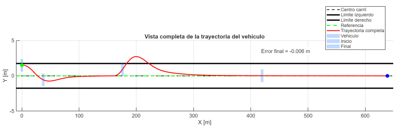
\includegraphics[width=0.85\textwidth]{Simulink_Respuesta.png}
    \caption{Respuesta del sistema de control de dirección ante un error lateral artificial simulado en MATLAB/Simulink. Error final: $-0{,}006$~m. Se aprecia la convergencia al centro del carril con oscilaciones amortiguadas.}
    \label{fig:simulink_respuesta}
\end{figure}

% ─────────────────────────────────────────────────────────────────────────────
\subsection{Parámetros del controlador}
% ─────────────────────────────────────────────────────────────────────────────

La Tabla~\ref{tab:pid} recoge los parámetros definitivos de ambos PIDs resultantes del proceso de sintonización. Estos valores se configuran directamente en el fichero \texttt{params.yaml} del paquete ROS2 y se cargan en tiempo de ejecución por el nodo \texttt{vehicle\_control\_node}.

\begin{table}[H]
    \centering
    \caption{Parámetros del controlador PID del sistema.}
    \label{tab:pid}
    \begin{tabular}{lcccc}
        \toprule
        \textbf{Controlador} & \textbf{Variable controlada} & $K_p$                   & $K_i$                   & $K_d$                   \\
        \midrule
        PID de dirección     & Error lateral (m)            & $2{,}00 \times 10^{-3}$ & $1{,}00 \times 10^{-3}$ & $1{,}07 \times 10^{-5}$ \\
        \bottomrule
    \end{tabular}
\end{table}

% ─────────────────────────────────────────────────────────────────────────────
\subsection{Transferibilidad de las ganancias}
% ─────────────────────────────────────────────────────────────────────────────

Una de las hipótesis de partida del trabajo es que las ganancias sintonizadas en MATLAB/Simulink son directamente transferibles a la implementación en Python/ROS2 sin necesidad de reajuste. Esta hipótesis se verifica experimentalmente en la Sección~\ref{sec:integracion}: el sistema opera correctamente a las velocidades de 18~km/h y 30~km/h con los mismos valores de $K_p$, $K_i$ y $K_d$ obtenidos en simulación, lo que confirma la validez del modelo utilizado para la sintonización y la coherencia entre el entorno MATLAB/Simulink y el simulador CARLA.

% ═════════════════════════════════════════════════════════════════════════════
\section{Integración en simulación y resultados}
\label{sec:integracion}
% ═════════════════════════════════════════════════════════════════════════════

Esta sección describe cómo los módulos de detección de carriles y control PID se integran en un sistema completo que opera en simulación en tiempo real. Se presentan el entorno de simulación empleado, la arquitectura software basada en ROS2, la infraestructura de contenedores Docker, los nodos que componen el sistema, la herramienta de monitorización y los resultados experimentales obtenidos.

% ─────────────────────────────────────────────────────────────────────────────
\subsection{Entorno de simulación: CARLA Simulator}
% ─────────────────────────────────────────────────────────────────────────────

Para el desarrollo y validación del sistema se ha empleado \textit{CARLA Simulator} (\textit{Car Learning to Act}), un simulador de conducción autónoma de código abierto basado en el motor gráfico \textit{Unreal Engine 4}. CARLA proporciona sensores virtuales de alta fidelidad —cámaras RGB, cámaras de segmentación semántica y medidores de velocidad— que permiten diseñar, depurar y validar algoritmos de percepción y control sin necesidad de un vehículo real.

El simulador se ejecuta en su versión \textit{0.9.15} dentro de un contenedor Docker con acceso a la GPU de la máquina anfitriona. Las principales características del entorno configurado son:

\begin{itemize}
    \item Mapa: Town04, escenario de carretera inter-urbana con marcas viales bien definidas.
    \item Vehículo (\textit{ego-vehicle}): modelo basado en el Tesla Model 3, controlado en lazo cerrado desde ROS2.
    \item Sensores disponibles:
          \begin{itemize}
              \item Cámara RGB frontal (\texttt{rgb\_front}): imagen principal usada para la detección de carriles.
              \item Cámara de segmentación semántica (\texttt{semantic\_segmentation\_front}): proporciona la máscara de \textit{ground truth} utilizada en la generación del dataset sintético.
              \item Medidor de velocidad (\texttt{speedometer}): velocidad actual del vehículo en m/s.
              \item Cámara exterior (\texttt{rgb\_view}): vista en tercera persona para supervisión visual.
          \end{itemize}
\end{itemize}

La Figura~\ref{fig:vistas_carla} muestra las dos perspectivas principales empleadas durante las sesiones de conducción autónoma.

\begin{figure}[H]
    \centering
    \begin{subfigure}[b]{0.48\textwidth}
        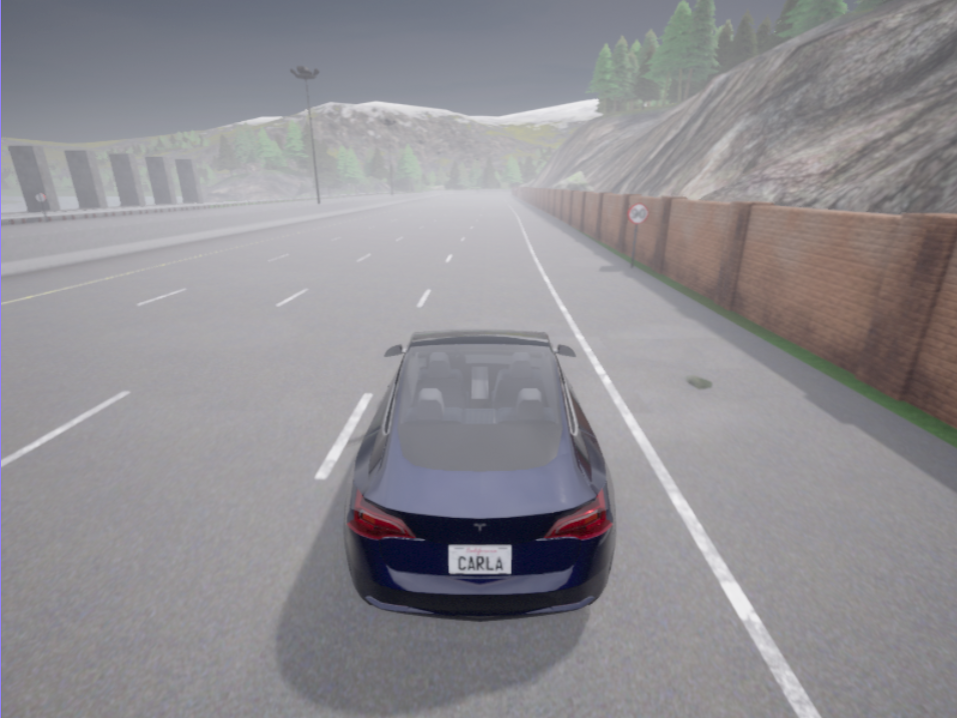
\includegraphics[width=\textwidth]{Vista_Externa.png}
        \caption{Vista exterior (tercera persona).}
    \end{subfigure}
    \hfill
    \begin{subfigure}[b]{0.48\textwidth}
        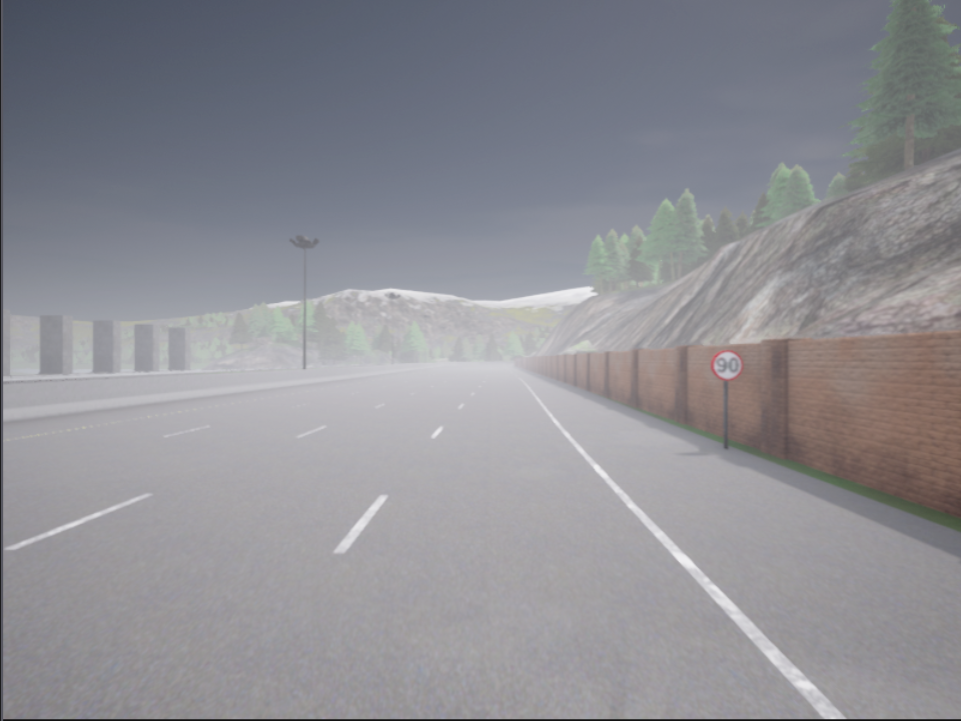
\includegraphics[width=\textwidth]{Vista_Camara_Frontal.png}
        \caption{Cámara frontal del vehículo.}
    \end{subfigure}
    \caption{Perspectivas en CARLA Simulator.}
    \label{fig:vistas_carla}
\end{figure}

% ─────────────────────────────────────────────────────────────────────────────
\subsection{Arquitectura del sistema}
% ─────────────────────────────────────────────────────────────────────────────

El sistema completo se organiza en tres capas que se comunican a través de una red Docker en modo \textit{host}:

\begin{enumerate}
    \item CARLA Simulator: simulador en su propio contenedor Docker con acceso a la GPU, que publica imágenes y telemetría como tópicos ROS2.
    \item CARLA-ROS2 Bridge: puente oficial (\texttt{carla\_ros\_bridge}) que traduce los datos de los sensores de CARLA en mensajes ROS2 estándar y convierte los comandos de control ROS2 en actuaciones sobre el vehículo simulado.
    \item Paquete de detección y control (\texttt{deteccion\_seguimiento\_carril}): paquete ROS2 propio que aloja los nodos de detección de carriles, control del vehículo y generación de anotaciones visuales.
\end{enumerate}

El flujo de datos es el siguiente: CARLA publica las imágenes de la cámara frontal en \texttt{/carla/ego\_vehicle/rgb\_front/image} y la velocidad en  \\ \texttt{/carla/ego\_vehicle/speedometer}. El \texttt{lane\_detection\_node} procesa cada \textit{frame} y publica el error lateral en metros en \texttt{/lane\_detection/lane\_error} y el estado completo del carril como JSON en \texttt{/lane\_detection/lane\_state}. El \texttt{vehicle\_control\_node} consume el error lateral y la velocidad para calcular y publicar los comandos de actuación en \texttt{/carla/ego\_vehicle/vehicle\_control\_cmd}. Por último, el \\ \texttt{annotation\_generator\_node} recoge el estado de todos los nodos y genera una capa de anotaciones visuales en \texttt{/foxglove/annotations}, que Foxglove Studio superpone sobre la imagen en tiempo real.

La Figura~\ref{fig:arquitectura} muestra el diagrama de bloques completo del sistema.

\begin{figure}[H]
    \centering
    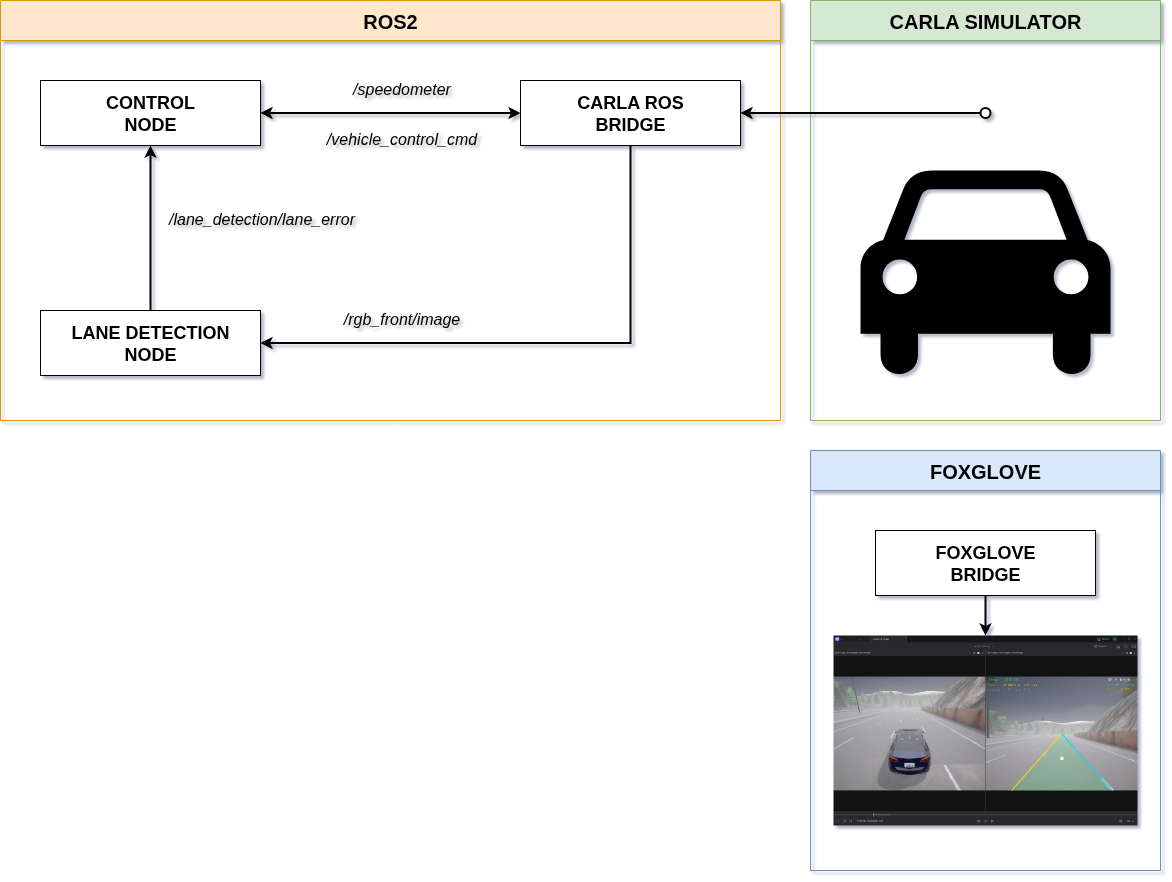
\includegraphics[width=0.95\textwidth]{diagram/Arquitectura.png}
    \caption{Diagrama de la arquitectura del sistema.}
    \label{fig:arquitectura}
\end{figure}

% ─────────────────────────────────────────────────────────────────────────────
\subsection{Infraestructura: Docker y contenedores}
% ─────────────────────────────────────────────────────────────────────────────

Todo el sistema se orquesta mediante \textbf{Docker Compose}, levantando los tres servicios con un único comando desde la raíz del repositorio:

\vspace{0.3cm}
\begin{lstlisting}[language=bash]
xhost +local:docker
docker compose -f tools/docker-compose.yaml up
\end{lstlisting}

La siguiente tabla describe cada uno de los servicios:

\begin{table}[H]
    \centering
    \label{tab:servicios_docker}
    \begin{tabular}{lll}
        \toprule
        \textbf{Servicio}    & \textbf{Contenedor}                     & \textbf{Función}                      \\
        \midrule
        \texttt{ros\_bridge} & \texttt{carla\_ros\_bridge}             & Bridge CARLA$\to$ROS2                 \\
        \texttt{navegacion}  & \texttt{deteccion\_seguimiento\_carril} & Lanzamiento del paquete de ROS2       \\
        \texttt{foxglove}    & \texttt{foxglove\_bridge}               & WebSocket bridge para Foxglove Studio \\
        \bottomrule
    \end{tabular}
\end{table}

La imagen Docker base es \texttt{ros:humble-ros-base-jammy}, sobre la que se instalan ROS2 Humble Hawksbill, las librerías de visión artificial (\texttt{python3-opencv}, \texttt{ros-humble-cv-bridge}), las herramientas de visualización (\texttt{ros-humble-foxglove-bridge}, \texttt{ros-humble-foxglove-msgs}) y el cliente Python de CARLA~0.9.15 junto con el \texttt{carla-ros-bridge} compilado desde el código fuente.

El código fuente del paquete ROS2 se monta como volumen dentro del contenedor de navegación. Esto permite que cualquier cambio en el host quede disponible tras ejecutar \texttt{colcon build --symlink-install} sin necesidad de reconstruir la imagen Docker.

% ─────────────────────────────────────────────────────────────────────────────
\subsection{Nodos ROS2 del sistema}
% ─────────────────────────────────────────────────────────────────────────────

El paquete \texttt{deteccion\_seguimiento\_carril} implementa tres nodos ROS2 en Python que se lanzan de forma conjunta mediante \texttt{run.launch.py}, más un nodo adicional de recolecta de datos que se activa por separado.

\subsubsection{Nodo de detección de carriles (\texttt{lane\_detection\_node})}

Este nodo recibe cada \textit{frame} de de la cámara frontal y ejecuta el pipeline de visión clásica descrito en la Sección~\ref{sec:carriles}. A partir de las líneas detectadas calcula el error lateral del vehículo respecto al centro del carril: primero en píxeles (\texttt{offset\_px}) y luego en metros, dividiendo por la longitud focal $f_x$ extraída del mensaje \texttt{camera\_info}. Los resultados se publican en:
\begin{itemize}
    \item \texttt{/lane\_detection/lane\_error} (\texttt{std\_msgs/Float32}): error lateral en metros.
    \item \texttt{/lane\_detection/lane\_state} (\texttt{std\_msgs/String}): JSON con las coordenadas de las líneas izquierda y derecha, la zona de posición (\texttt{CENTER}/\texttt{LEFT}/\texttt{RIGHT}) y los flags de detección.
\end{itemize}

\subsubsection{Nodo de control del vehículo (\texttt{vehicle\_control\_node})}

Este nodo cierra el lazo de control: recibe el error lateral y la velocidad actual, y genera los comandos de actuación sobre el vehículo. Opera a 20~Hz e implementa dos controladores PID independientes.

\paragraph{PID de velocidad (control de crucero).}
Regula la velocidad del vehículo en torno a la referencia configurable \texttt{target\_speed}. El error de control es la diferencia entre la velocidad objetivo y la medida por el velocímetro. La salida del PID se mapea a los canales \textit{throttle} (acelerador) y \textit{brake} (freno) normalizados en $[0, 1]$:

\begin{align}
    e_v(t)          & = v_{\text{ref}} - v_{\text{actual}} \notag          \\
    u_v(t)          & = K_{p,v}\,e_v + K_{i,v}\int e_v\,\mathrm{d}t \notag \\
    \text{throttle} & = \max(0,\,\min(1,\, u_v)), \quad
    \text{brake} = \max(0,\,\min(1,\,-u_v)) \notag
\end{align}

\paragraph{PID de dirección (mantenimiento de carril).}
Ajusta el ángulo del volante para mantener el vehículo centrado en el carril. El PID opera en radianes y su salida se normaliza por el ángulo físico máximo del volante ($\theta_{\max} = 0.6~\text{rad} \approx 34^\circ$) para obtener el valor de dirección normalizado de CARLA en $[-1,1]$. La convención de signo es: error positivo (vehículo desplazado a la derecha) produce una corrección hacia la izquierda (steer~$< 0$):

\begin{align}
    u_s(t)       & = K_{p,s}\,e_s + K_{i,s}\int e_s\,\mathrm{d}t + K_{d,s}\,\dot{e}_s \notag         \\
    \text{steer} & = \max\!\left(-1,\,\min\!\left(1,\,\frac{u_s}{\theta_{\max}}\right)\right) \notag
\end{align}

Ambos PIDs incorporan \textit{anti-windup} que limita el término integral al rango $[-10, 10]$. Los parámetros definitivos configurados en \texttt{params.yaml} se recogen en la Tabla~\ref{tab:pid}. Estos valores son el resultado de la sintonización en MATLAB/Simulink descrita en la Sección~\ref{sec:control}, trasladados directamente a la implementación en Python.

\subsubsection{Nodo generador de anotaciones (\texttt{annotation\_generator\_node})}

Este nodo actúa como capa de visualización del sistema. En cada \textit{frame} de la cámara frontal recoge el estado de los demás nodos y genera un mensaje \\ \texttt{foxglove\_msgs/ImageAnnotations} que Foxglove Studio superpone sobre la imagen en tiempo real. Las anotaciones incluyen:

\begin{itemize}
    \item Polígono de carril: región semitransparente en verde que cubre el área delimitada por las líneas izquierda y derecha detectadas.
    \item Líneas de carril: línea izquierda en amarillo y derecha en cian, con grosor de 5~px.
    \item Vector de desviación: segmento desde el centro geométrico de la imagen hasta el centro estimado del carril, en amarillo.
    \item HUD de telemetría: zona del carril (\texttt{CENTER}/\texttt{LEFT}/\texttt{RIGHT}), error lateral en metros y en píxeles, velocidad actual en km/h, y valores de \textit{throttle}, \textit{brake} y \textit{steer}.
\end{itemize}

La Figura~\ref{fig:interfaz} muestra la interfaz de Foxglove Studio durante una sesión de conducción.

\begin{figure}[H]
    \centering
    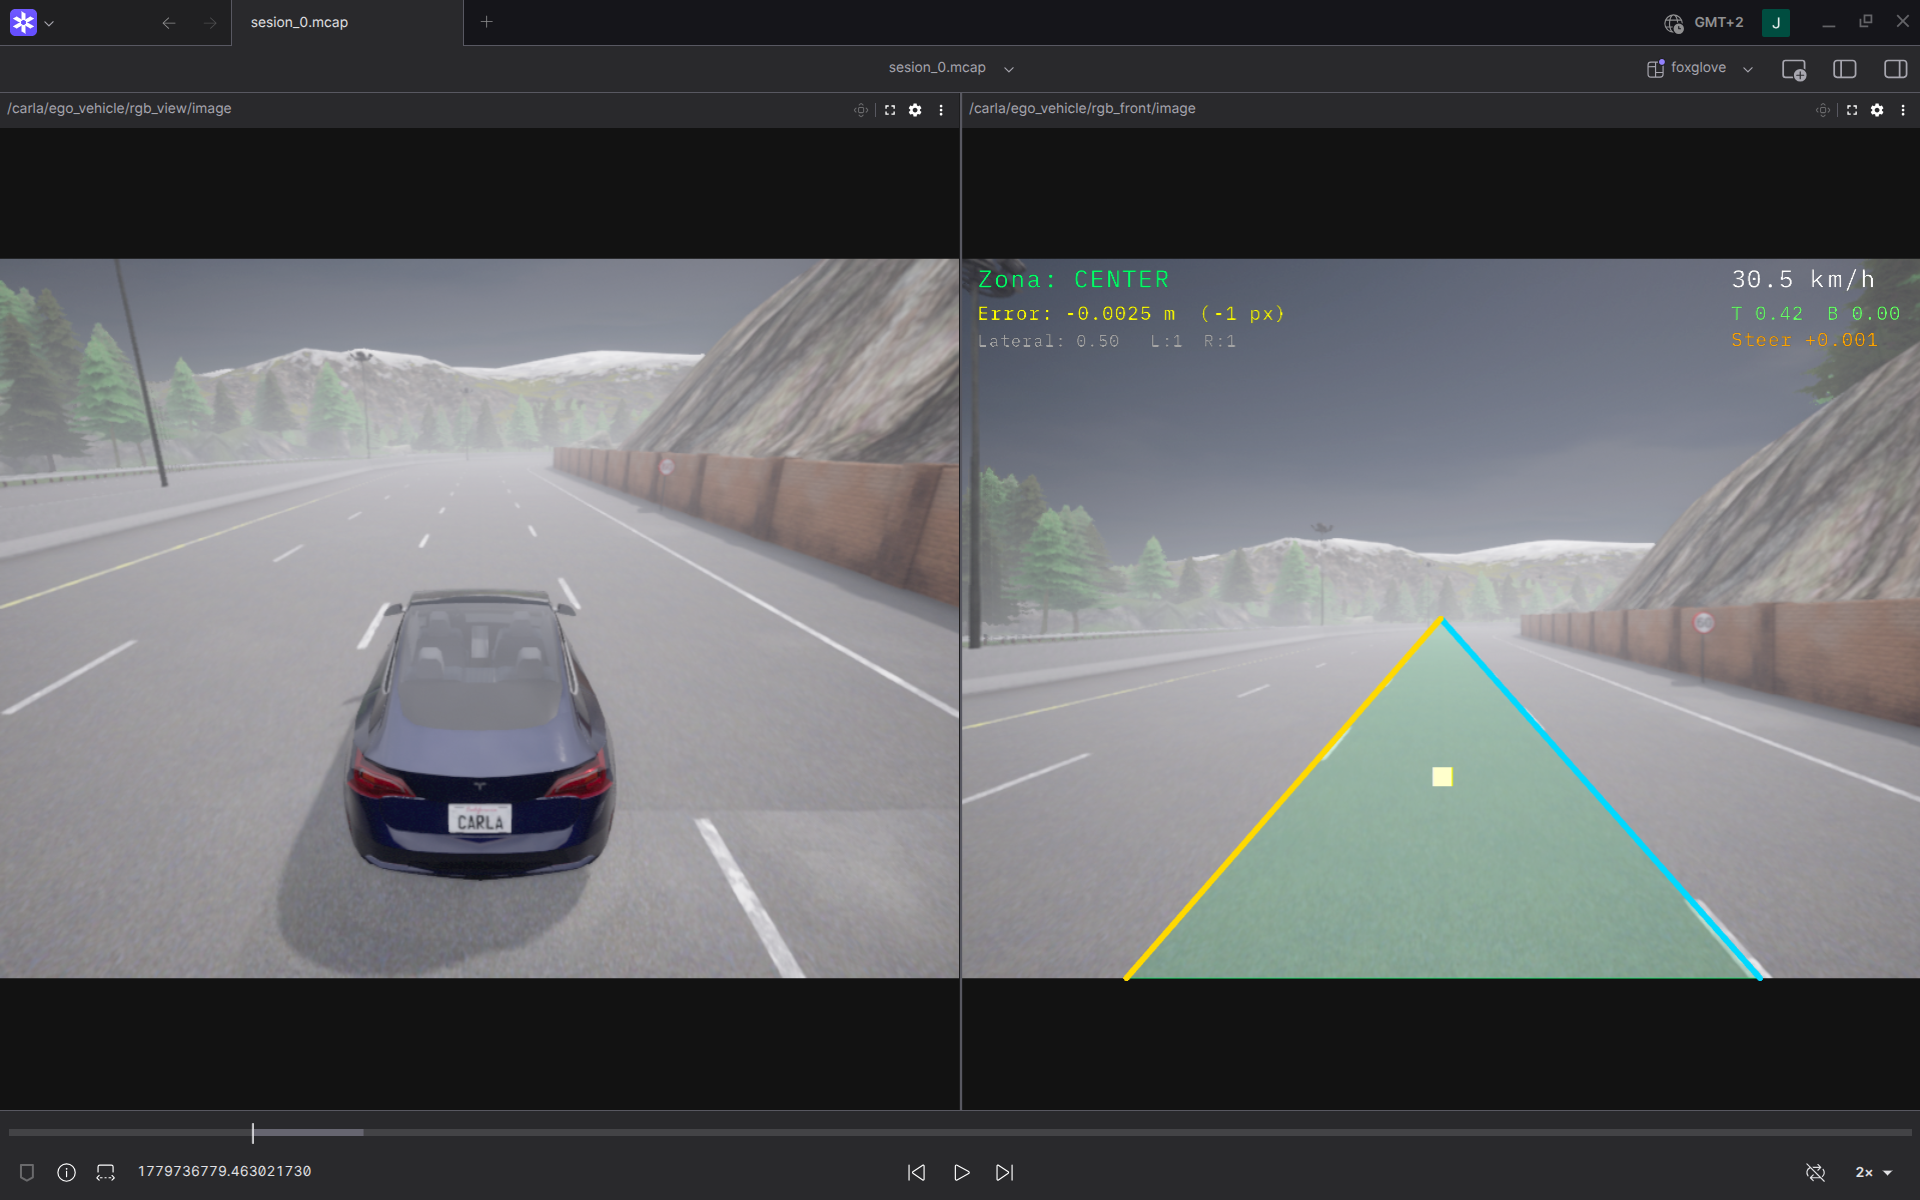
\includegraphics[width=\textwidth]{Interfaz.png}
    \caption{Interfaz de Foxglove Studio durante una sesión de conducción autónoma. A la izquierda, la vista exterior del vehículo; a la derecha, la cámara frontal con las anotaciones superpuestas: líneas del carril, polígono de área y HUD de telemetría.}
    \label{fig:interfaz}
\end{figure}

% ─────────────────────────────────────────────────────────────────────────────
\subsection{Generación de datasets sintéticos}
% ─────────────────────────────────────────────────────────────────────────────

Una de las ventajas de trabajar con un simulador como CARLA es la posibilidad de generar datos etiquetados de forma automática. La cámara de segmentación semántica asigna a cada píxel una etiqueta de clase con precisión perfecta, ofreciendo un \textit{ground truth} ideal para evaluar el detector de carriles sin ningún coste de anotación manual.

El nodo \texttt{lane\_dataset\_node} opera en modo conducción manual (sin el nodo de control) y captura imágenes a 5~Hz. Para cada instante capturado:
\begin{enumerate}
    \item Obtiene la máscara semántica del mismo instante de tiempo.
    \item Detecta los píxeles de marcas viales en la máscara y los proyecta sobre la imagen RGB.
    \item Almacena el par imagen~RGB / máscara binaria en \texttt{dataset/lanes/images/} y \texttt{dataset/lanes/masks/} respectivamente.
\end{enumerate}

La recolecta se lanza con:
\vspace{0.3cm}
\begin{lstlisting}[language=bash]
xhost +local:docker
docker compose -f tools/docker-compose-lane-dataset.yaml up
\end{lstlisting}

El repositorio incluye además la herramienta \texttt{tools/visualize\_lanes\_dataset.py} para revisar el dataset generado y \texttt{tools/make\_lane\_video.py} para producir un vídeo con el detector de carriles aplicado sobre las imágenes del dataset.

% ─────────────────────────────────────────────────────────────────────────────
\subsection{Resultados}
% ─────────────────────────────────────────────────────────────────────────────

Las pruebas de conducción autónoma se han realizado a dos velocidades de referencia: 18~km/h (5.0~m/s) y 30~km/h (8.33~m/s), modificando únicamente el parámetro \texttt{target\_speed} en \texttt{params.yaml}. En ambos casos el sistema es capaz de mantener el vehículo centrado en el carril de forma continuada sin intervención humana.

Los vídeos de las sesiones de conducción autónoma a 18~km/h y 30~km/h, así como un vídeo de demostración del detector de carriles sobre el dataset sintético, están disponibles en el repositorio público de GitHub:

\begin{center}
    \url{https://github.com/JoseLopez36/Deteccion-Seguimiento-Carril}
\end{center}

Los ficheros correspondientes son \texttt{media/Demo\_18\_kmh.mp4}, \texttt{media/Demo\_30\_kmh.mp4} y \texttt{media/Deteccion\_Carriles.mp4}.

% ═════════════════════════════════════════════════════════════════════════════
\section{Conclusiones}
% ═════════════════════════════════════════════════════════════════════════════

Este trabajo ha permitido implementar un sistema de \textit{Lane Keeping Assist} funcional de extremo a extremo, demostrando que la combinación de técnicas de visión clásica con un controlador PID en cascada y una arquitectura ROS2 modular constituye una solución eficaz y fácilmente reproducible para la conducción autónoma en simulación.

% TODO

\end{document}